\documentclass[]{article}

\usepackage{cite} % For citations
\usepackage[backref]{hyperref} % For hyperlinks and references
\usepackage{amsmath} % For math expressions
\usepackage{graphicx} % For including graphics
\usepackage{fancyhdr} % For custom headers and footers
\usepackage{subcaption} % For subfigures
\usepackage{float} % For better figure placement control

\title{\textbf{Computer Vision homework 4}}
\author{Pan Changxun}
\date{May 2025}

\topmargin=-0.45in      %
\evensidemargin=0in     %
\oddsidemargin=0in      %
\textwidth=6.5in   
\textheight=9.0in       %
\headsep=0.25in 

\pagestyle{fancy}
\fancyhf{} % Clear all header and footer fields
\fancyhead[L]{Pan Changxun} % Left header
\fancyhead[C]{Computer Vision homework 4} % Center header
\fancyhead[R]{May 2025} % Right header
%\fancyfoot[L]{\leftmark} % Left footer
\fancyfoot[C]{\thepage} % Center footer
%\fancyfoot[R]{} % Right footer

\begin{document}
\maketitle

\section{Models}
I first tried to use the UNet model, but it did not perform well for this segmentation task. I then implemented the DeepLabV3 model and further improved it to DeepLabV3+. The DeepLabV3+ architecture consists of the following key components:

\begin{itemize}
    \item A backbone network using ResNet with atrous convolutions
    \item Atrous Spatial Pyramid Pooling (ASPP) to capture multi-scale context
    \item A decoder module that refines the segmentation results
    \item Skip connections that combine low-level features with high-level features
\end{itemize}

This architecture is particularly effective for semantic segmentation tasks as it captures both detailed spatial information and broad contextual information.

\subsection{Model Architecture Details}
The DeepLabV3+ model I implemented consists of several carefully designed components:

\subsubsection{ResNet Backbone}
I implemented a custom ResNet backbone with atrous (dilated) convolutions:
\begin{itemize}
    \item Initial layer: 7×7 convolution with stride 2, followed by batch normalization, ReLU, and max pooling
    \item Layer 1: 3 ResNet blocks with 64 channels
    \item Layer 2: 4 ResNet blocks with 128 channels, stride 2
    \item Layer 3: 6 ResNet blocks with 256 channels, dilation rate 2
    \item Layer 4: 3 ResNet blocks with 512 channels, dilation rate 4
\end{itemize}

Each ResNet block consists of two 3×3 convolutional layers with batch normalization and ReLU, along with a residual connection. The increasing dilation rates in deeper layers ensure a larger receptive field without decreasing spatial resolution.

\subsubsection{ASPP Module}
The Atrous Spatial Pyramid Pooling module consists of:
\begin{itemize}
    \item One 1×1 convolution
    \item Three 3×3 atrous convolutions with dilation rates of 12, 24, and 36
    \item A global average pooling branch followed by a 1×1 convolution
\end{itemize}

These five branches are concatenated and fed through a 1×1 convolution with 256 output channels, followed by batch normalization, ReLU, and a dropout layer (rate=0.5) to obtain the final ASPP features.

\subsubsection{Decoder Module}
The decoder integrates the semantically rich features from the ASPP module with spatially detailed low-level features from earlier layers:
\begin{itemize}
    \item Low-level features from the first ResNet layer are processed by a 1×1 convolution to reduce channels to 48
    \item ASPP features are upsampled to match the spatial dimensions of the low-level features
    \item Both feature maps are concatenated and processed by two 3×3 convolutions
    \item The result is then upsampled to input resolution and fed to a final classifier
\end{itemize}

\subsubsection{Final Classification Layer}
A simple 1×1 convolution transforms the decoder output into class logits with 19 channels (one for each class in the Cityscapes dataset).

\subsubsection{Weight Initialization}
All convolutional layers use Kaiming initialization to ensure proper gradient flow during training, while batch normalization layers are initialized with weight=1 and bias=0.

\subsection{Model Implementation Details}

\subsubsection{Forward Pass Process}
The forward pass through the model is implemented as follows:
\begin{enumerate}
    \item Input image is processed by the ResNet backbone
    \item Encoder produces high-level features (output of layer 4) and low-level features (output of layer 1)
    \item High-level features are passed through the ASPP module for multi-scale context extraction
    \item ASPP features and low-level features are combined in the decoder module
    \item Final classifier converts the feature map to logits
    \item Output is upsampled to input resolution using bilinear interpolation
\end{enumerate}

\subsubsection{Key Implementation Components}

\paragraph{Atrous (Dilated) Convolutions}
I used dilated convolutions to increase the receptive field without increasing the number of parameters or reducing the spatial resolution. In standard convolutions, the filter elements are applied to adjacent input elements. In dilated convolutions, gaps ("holes") are introduced between filter elements, effectively increasing the receptive field while maintaining the same number of parameters.

For example, with a dilation rate of 2, each filter element applies to inputs that are 2 pixels apart, effectively doubling the receptive field without increasing the filter size. This is crucial for semantic segmentation where both global context and fine details need to be preserved.

\paragraph{ASPP Design Considerations}
The ASPP module captures multi-scale information through parallel atrous convolutions with different dilation rates (12, 24, and 36). These different rates allow the network to capture context at various scales:
\begin{itemize}
    \item Smaller dilation rates: capture fine details and local context
    \item Larger dilation rates: capture broader context and object relationships
    \item Global average pooling branch: captures image-level context
\end{itemize}

\paragraph{Skip Connection Implementation}
The skip connection between the encoder and decoder is crucial for recovering spatial details lost during downsampling. By connecting the low-level features from the first ResNet block to the decoder, the model can combine semantic information (from deep layers) with spatial information (from shallow layers), resulting in more accurate boundary delineation.

The low-level features undergo a 1×1 convolution to reduce the channel dimension from 64 to 48, making the fusion more balanced and computationally efficient.

\section{Experiments}
\subsection{Initial Training without Cross-Validation}
I initially conducted experiments without cross-validation to establish a baseline. However, I observed that the model quickly began to overfit, with the loss no longer decreasing after a certain point. Despite this limitation, the model achieved a mean Intersection over Union (mIoU) of approximately 51\%. The training curve is shown in Figure~\ref{fig:no_cross_val_10_30}.

\subsection{Cross-Validation Training Strategy}
To address the overfitting issue, I implemented a 5-fold cross-validation approach by splitting the training set. This significantly improved performance, with the mIoU reaching approximately 58\% by the end of training.

The training schedule was designed as follows:
\begin{itemize}
    \item First 30 epochs: learning rate = $1 \times 10^{-4}$
    \item Epochs 30-50: initial learning rate = $5 \times 10^{-5}$
\end{itemize}

For learning rate adjustment, I used the Plateau scheduling method, which reduces the learning rate by a factor of 0.5 if the mIoU does not improve over 5 consecutive epochs.

After training all folds, I evaluated three model aggregation approaches:
\begin{enumerate}
    \item The best mIoU model from all folds
    \item The average of parameters from the best models across all folds
    \item The average of parameters from the top 3 best mIoU models across all folds
\end{enumerate}

The best performing model from these three approaches was then used as the pre-trained model for the next 20-epoch training iteration. Since the initial training was for 10 epochs, subsequent training stages began at epochs 10, 30, 50, etc.

The results for the first cross-validation stage (epochs 10-30) are shown in Figures~\ref{fig:cross_val_10_30_combined} and \ref{fig:cross_val_10_30_val}. Figure~\ref{fig:cross_val_10_30_combined} shows the training curves and IoU progression for fold 1, while Figure~\ref{fig:cross_val_10_30_val} compares mIoU across all folds on the official validation set.

\subsection{Training Results for Epochs 30-50}
During the second training phase (epochs 30-50), I observed a slight decrease in overall performance. However, the averaged model still maintained a respectable mIoU of 54\%, indicating the robustness of the model averaging approach. The training performance for this stage is illustrated in Figures~\ref{fig:cross_val_30_50_combined} and \ref{fig:cross_val_30_50_val}. Figure~\ref{fig:cross_val_30_50_combined} presents the training curves and IoU progression for fold 1, while Figure~\ref{fig:cross_val_30_50_val} shows the mIoU comparison across all folds.


\subsection{Training Results for Epochs 50-70}
Encouragingly, performance improved during the third training phase (epochs 50-70), with the best model achieving an mIoU of 56\%. This improvement suggests that the learning rate adjustment strategy and continued training were effective in refining the model parameters. The results of this training phase are presented in Figures~\ref{fig:cross_val_50_70_combined} and \ref{fig:cross_val_50_70_val}, showing the detailed performance metrics across different folds.



\subsection{Final Optimization and Results}
For final optimization, I implemented a cosine learning rate scheduler, which further improved performance. With this approach, the best model achieved an mIoU of approximately 58\%, although there was considerable variance across folds. Given the performance plateau and the significant variance, I decided to conclude the training at this point.

The final test results are presented in Figures~\ref{fig:per_class_iou}, \ref{fig:confusion_matrix}, and \ref{fig:class_weight_vs_iou}, with detailed visualizations available in the directory \texttt{outputs/deeplabv3plus\_test\_results}. Figure~\ref{fig:per_class_iou} shows the per-class IoU scores, Figure~\ref{fig:confusion_matrix} presents the confusion matrix for segmentation results, and Figure~\ref{fig:class_weight_vs_iou} illustrates the relationship between class weights and IoU scores.

\section{Figures}

\begin{figure}[htbp]
		\centering
		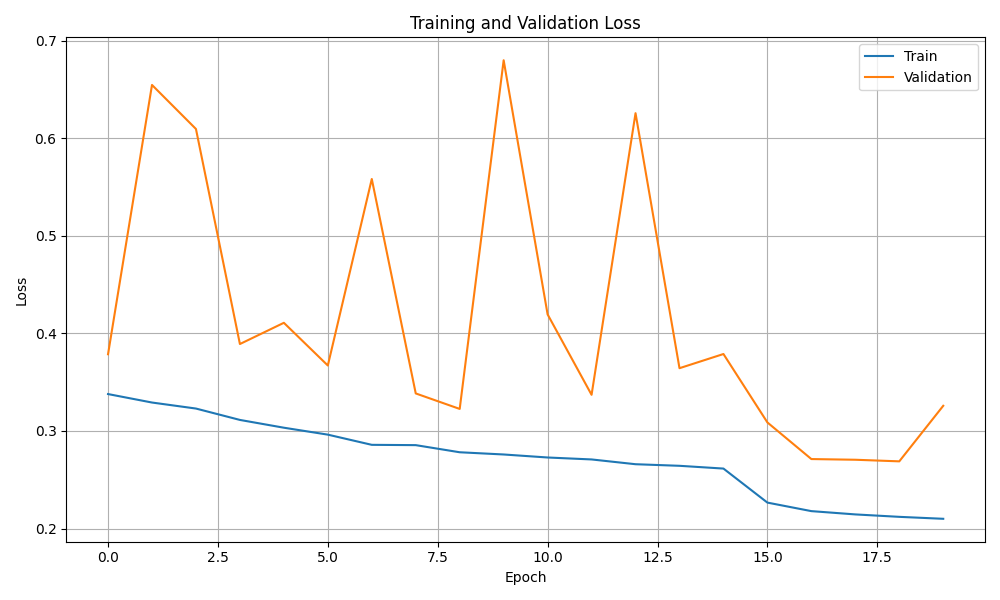
\includegraphics[width=0.8\textwidth]{no_cross_val_10_30.png}
		\caption{Training curve for epochs 10 to 30 without cross-validation, showing signs of overfitting}
		\label{fig:no_cross_val_10_30}
\end{figure}

\begin{figure}[htbp]
    \centering
    \begin{subfigure}[b]{0.8\textwidth}
        \centering
        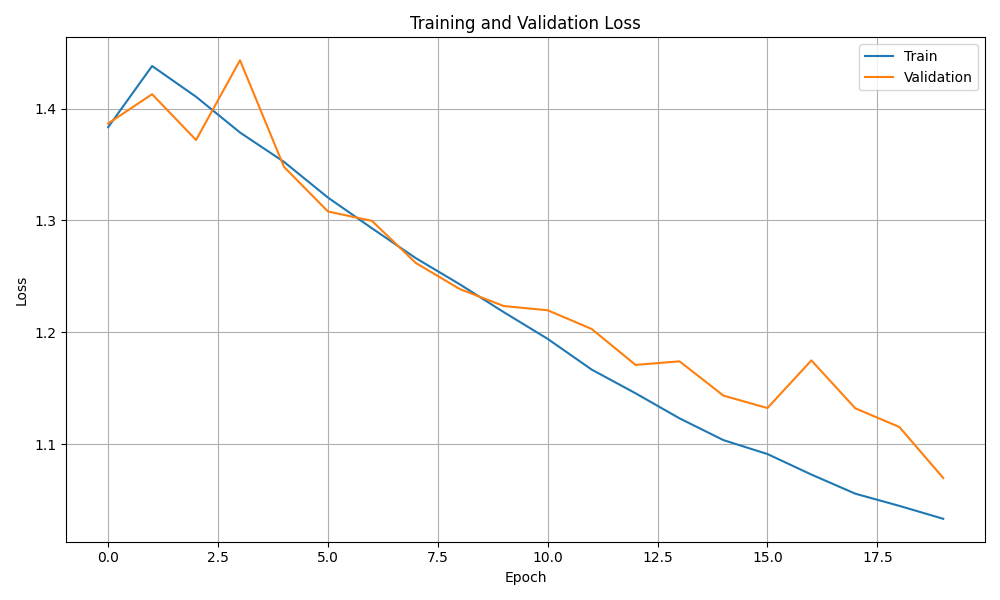
\includegraphics[width=\textwidth]{cross_10_30.png}
        \caption{Training curves for fold 1, epochs 10-30}
        \label{fig:cross_val_10_30}
    \end{subfigure}
    \vspace{0.5cm}
    \begin{subfigure}[b]{0.8\textwidth}
        \centering
        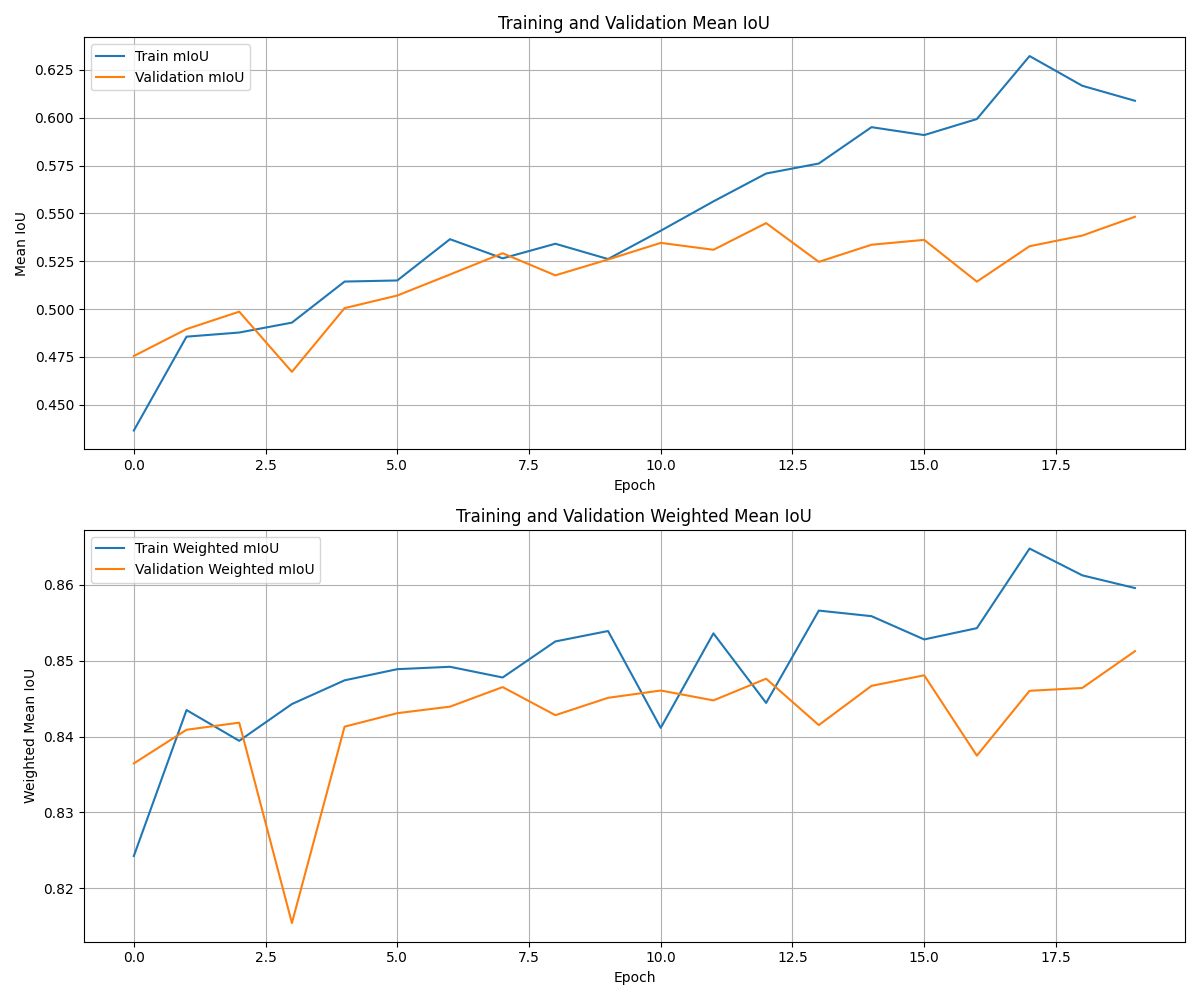
\includegraphics[width=\textwidth]{iou_history_cross_10_30.png}
        \caption{IoU progression history for fold 1, epochs 10-30}
        \label{fig:cross_val_10_30_iou_his}
    \end{subfigure}
    \caption{Training performance for the first cross-validation stage (epochs 10-30)}
    \label{fig:cross_val_10_30_combined}
\end{figure}

\begin{figure}[htbp]
    \centering
    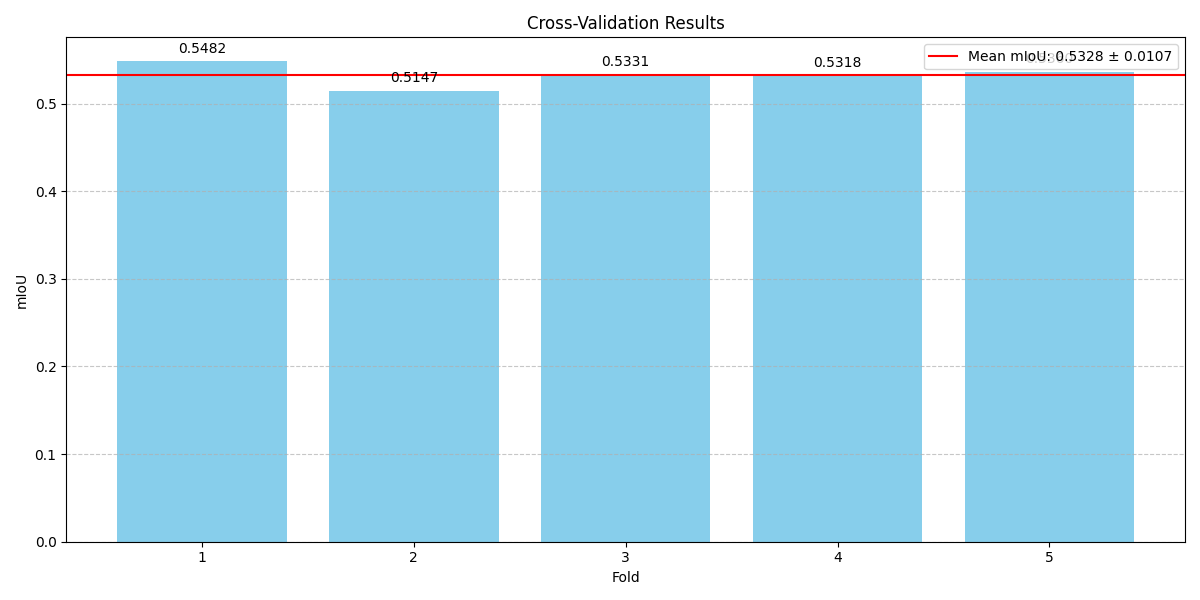
\includegraphics[width=0.8\textwidth]{folds_10_30.png}
    \caption{mIoU comparison across all folds on the official validation set, epochs 10-30}
    \label{fig:cross_val_10_30_val}
\end{figure}

\begin{figure}[htbp]
    \centering
    \begin{subfigure}[b]{0.8\textwidth}
        \centering
        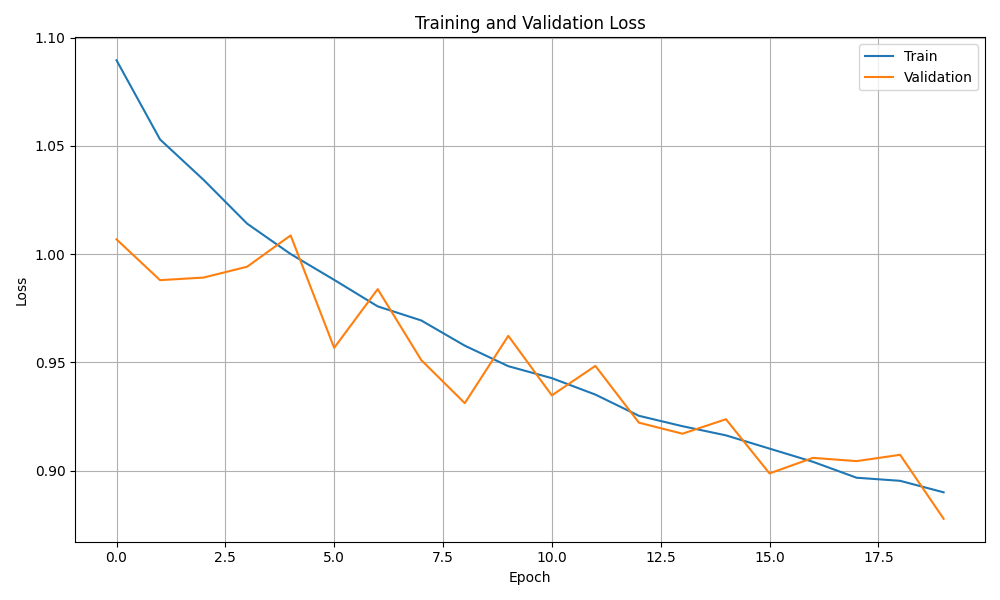
\includegraphics[width=\textwidth]{cross_30_50.png}
        \caption{Training curves for fold 1, epochs 30-50}
        \label{fig:cross_val_30_50}
    \end{subfigure}
    \vspace{0.5cm}
    \begin{subfigure}[b]{0.8\textwidth}
        \centering
        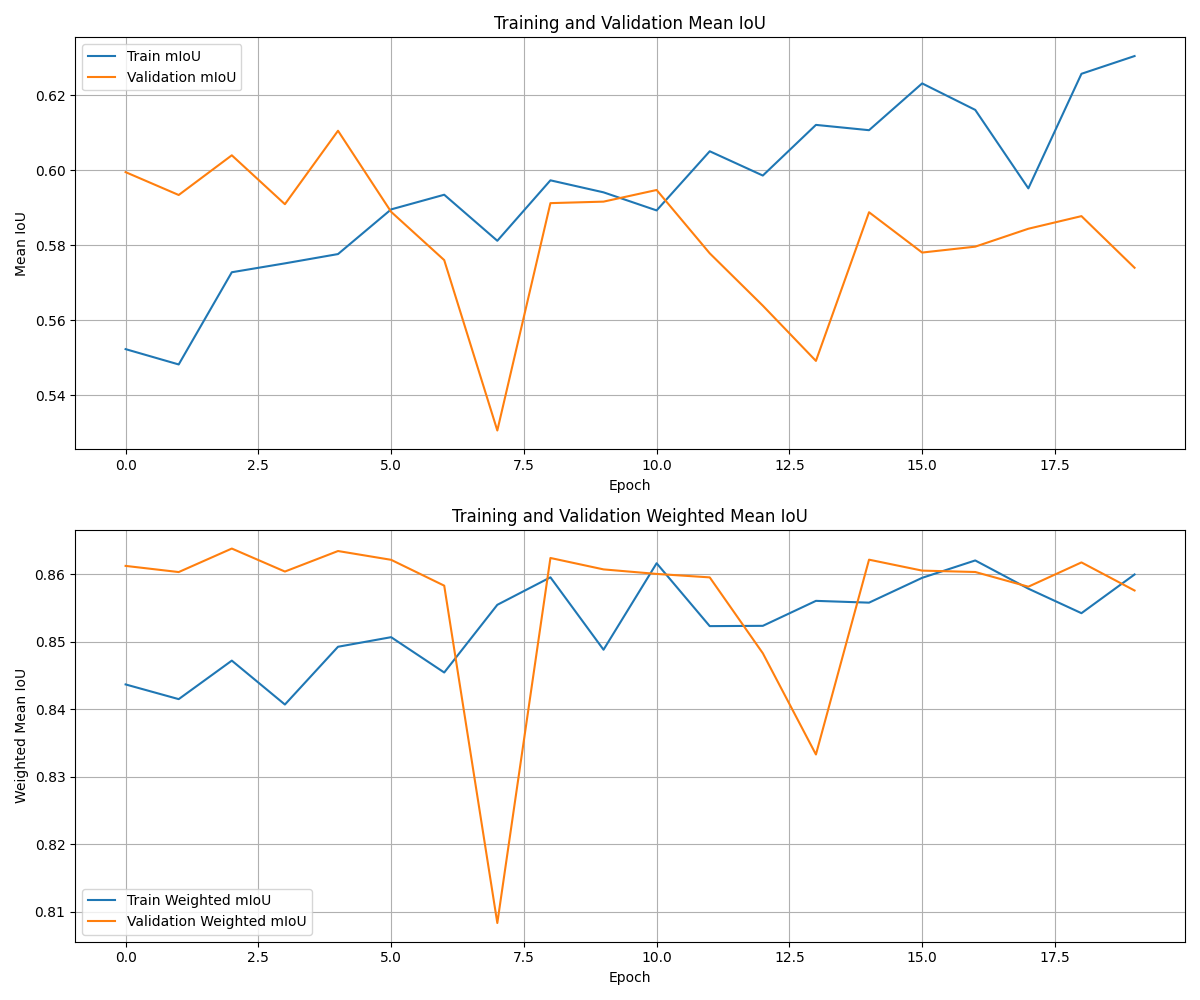
\includegraphics[width=\textwidth]{iou_history_cross_30_50.png}
        \caption{IoU progression history for fold 1, epochs 30-50}
        \label{fig:cross_val_30_50_iou_his}
    \end{subfigure}
    \caption{Training performance for the second cross-validation stage (epochs 30-50)}
    \label{fig:cross_val_30_50_combined}
\end{figure}

\begin{figure}[htbp]
    \centering
    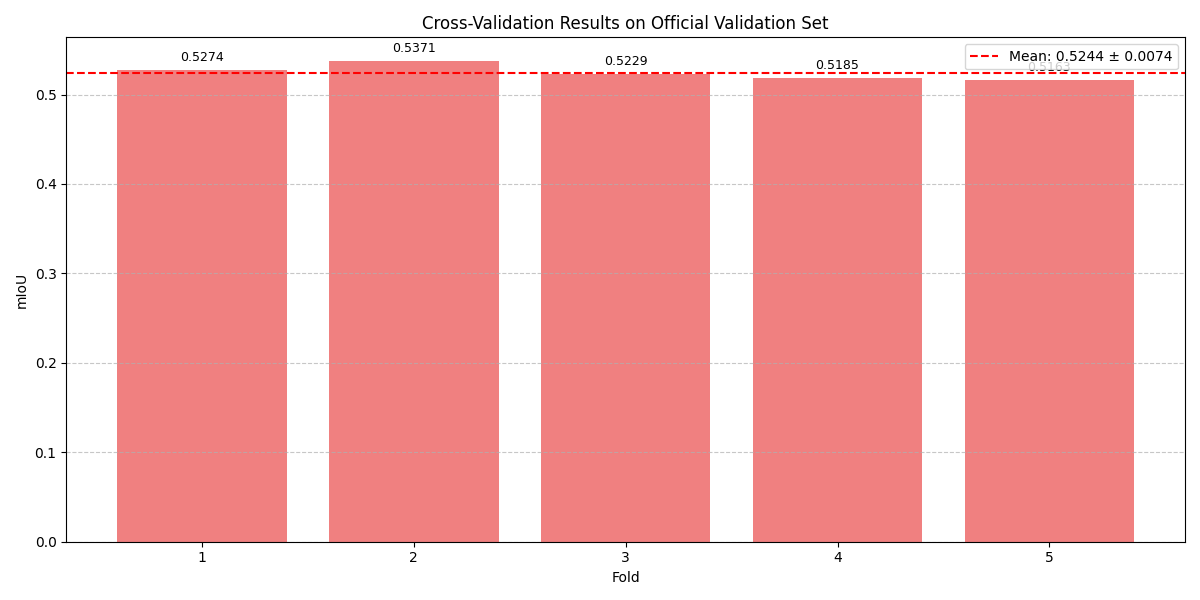
\includegraphics[width=0.8\textwidth]{folds_30_50.png}
    \caption{mIoU comparison across all folds on the official validation set, epochs 30-50}
    \label{fig:cross_val_30_50_val}
\end{figure}

\begin{figure}[htbp]
    \centering
    \begin{subfigure}[b]{0.8\textwidth}
        \centering
        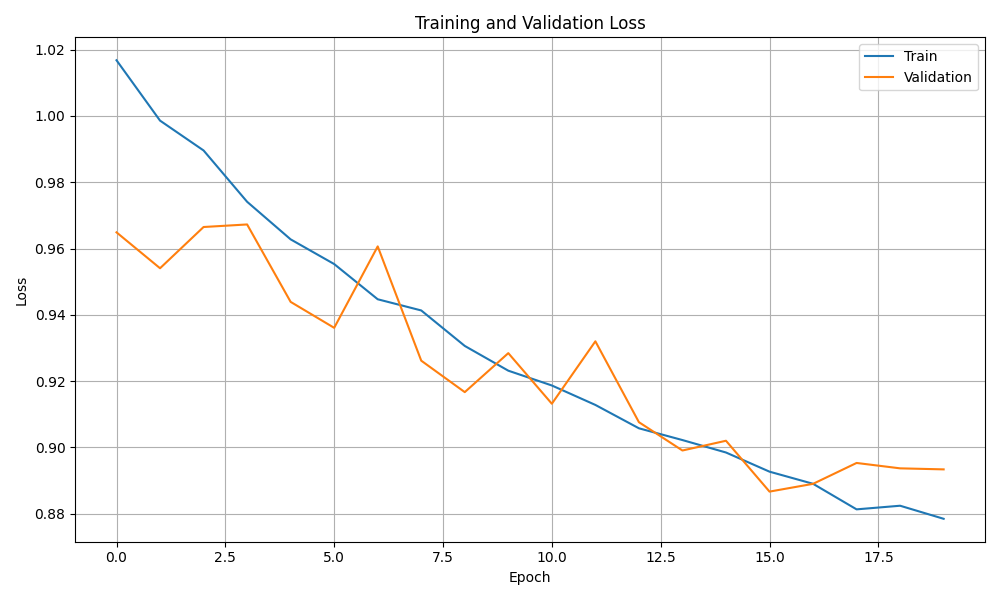
\includegraphics[width=\textwidth]{cross_50_70.png}
        \caption{Training curves for fold 1, epochs 50-70}
        \label{fig:cross_val_50_70}
    \end{subfigure}
    \vspace{0.5cm}
    \begin{subfigure}[b]{0.8\textwidth}
        \centering
        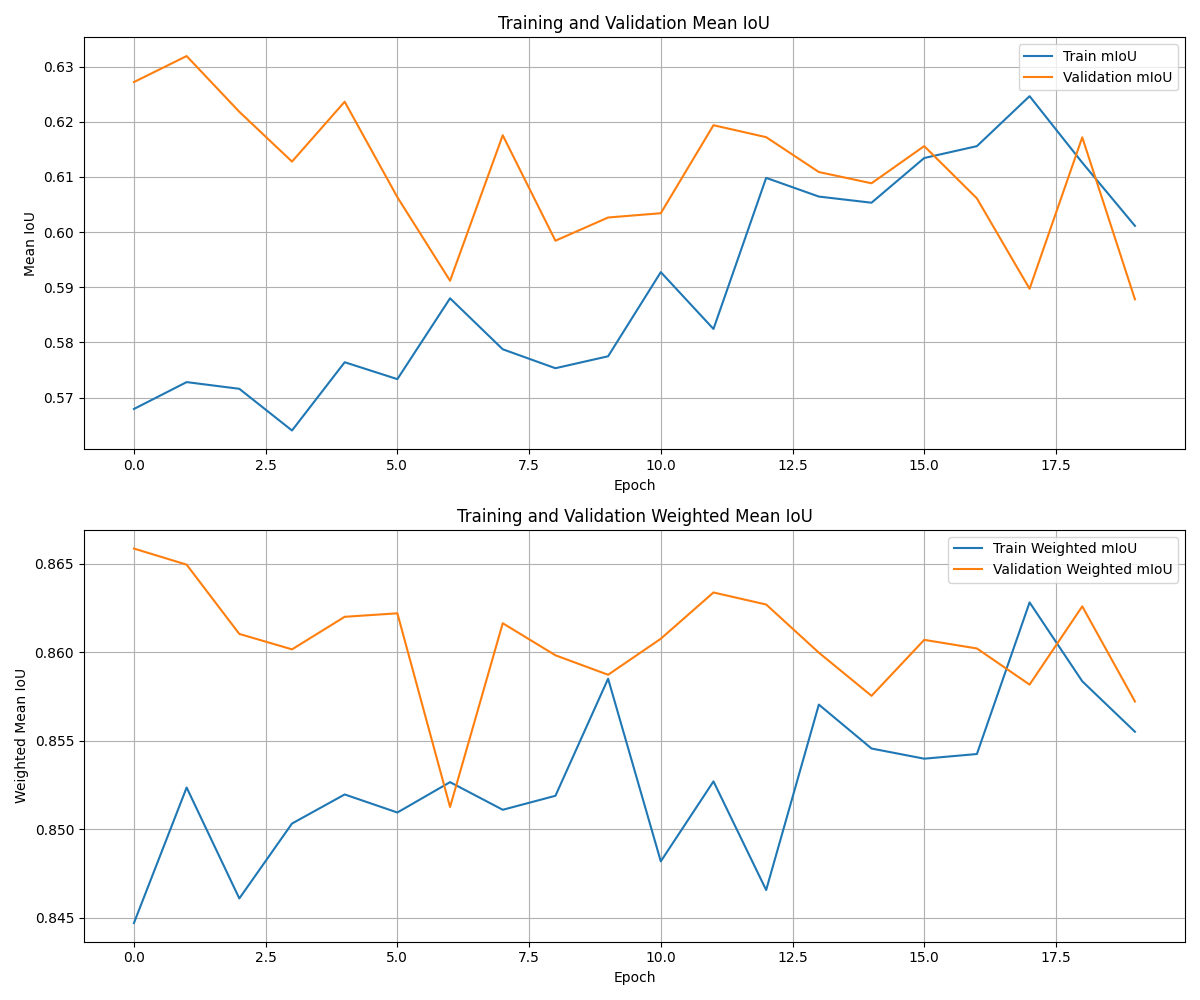
\includegraphics[width=\textwidth]{iou_history_cross_50_70.png}
        \caption{IoU progression history for fold 1, epochs 50-70}
        \label{fig:cross_val_50_70_iou_his}
    \end{subfigure}
    \caption{Training performance for the third cross-validation stage (epochs 50-70)}
    \label{fig:cross_val_50_70_combined}
\end{figure}

\begin{figure}[htbp]
    \centering
    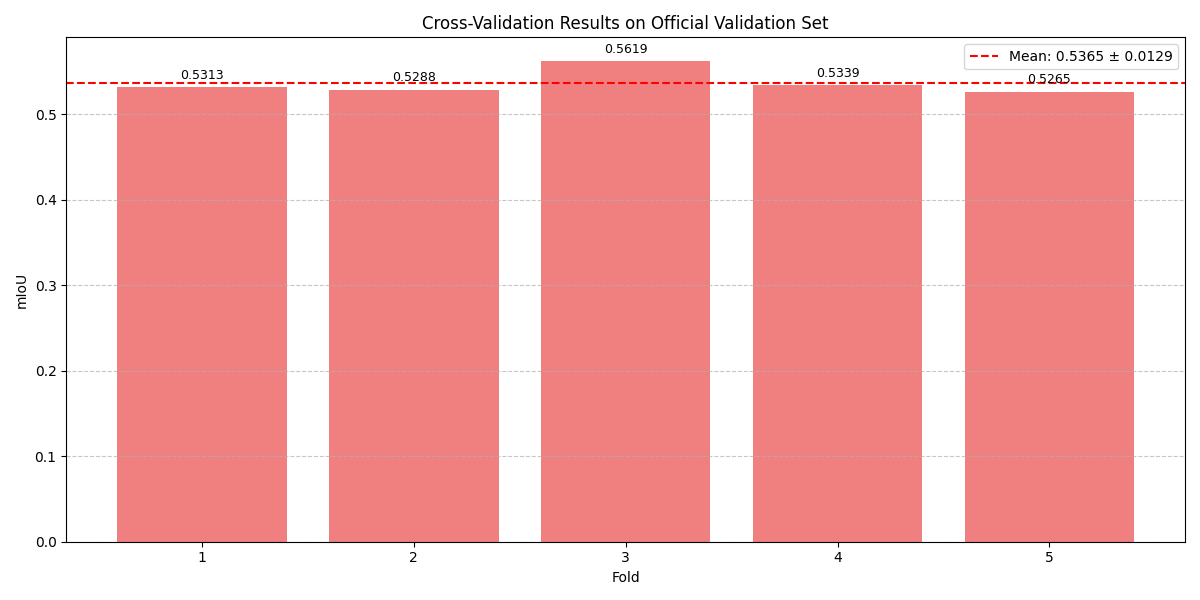
\includegraphics[width=0.8\textwidth]{folds_50_70.png}
    \caption{mIoU comparison across all folds on the official validation set, epochs 50-70}
    \label{fig:cross_val_50_70_val}
\end{figure}

\begin{figure}[htbp]
    \centering
    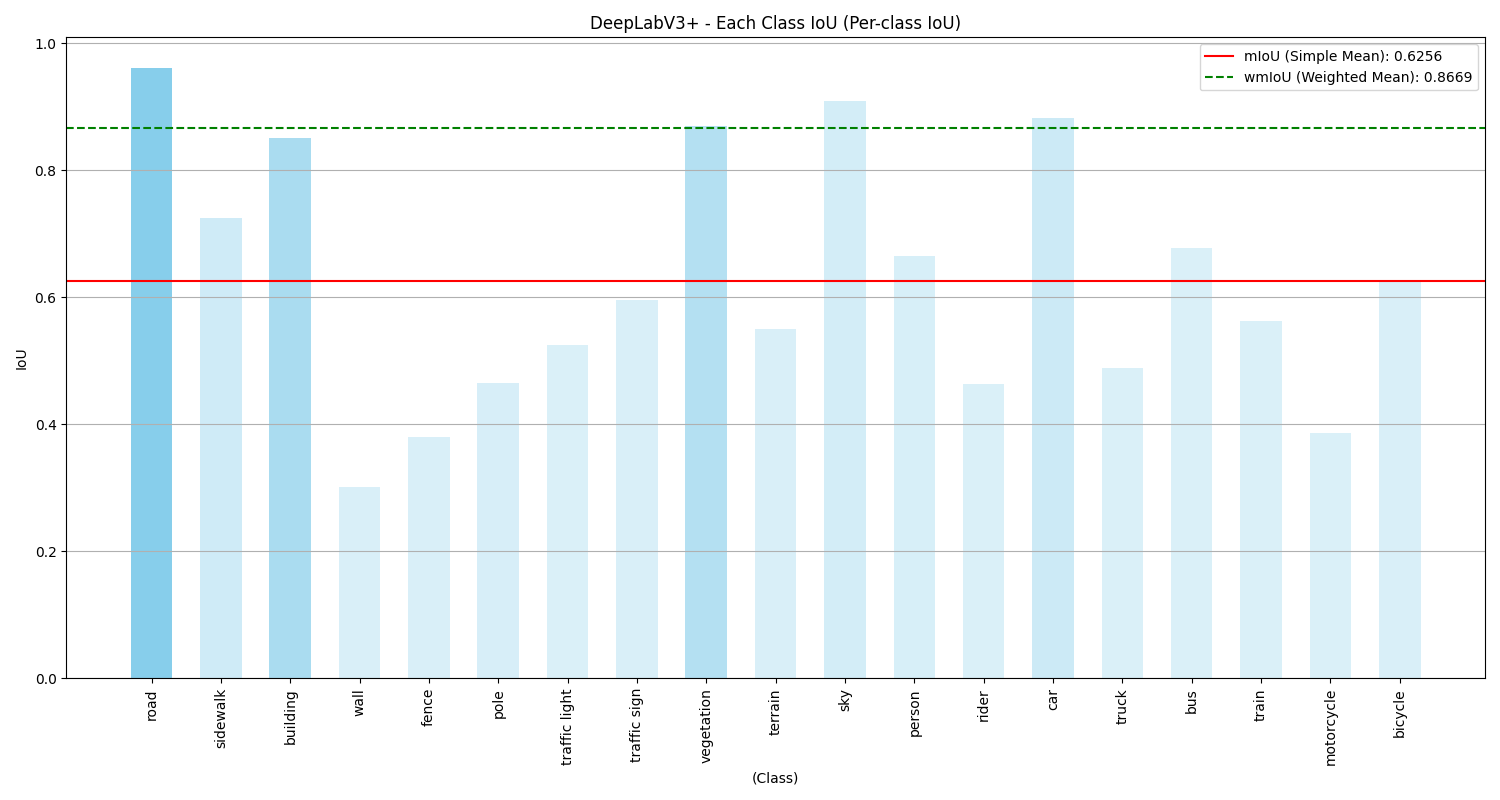
\includegraphics[width=0.8\textwidth]{outputs/deeplabv3plus_test_results/per_class_iou.png}
    \caption{Per-class IoU scores for the final model, showing the model's performance across different semantic categories}
    \label{fig:per_class_iou}
\end{figure}

\begin{figure}[htbp]
    \centering
    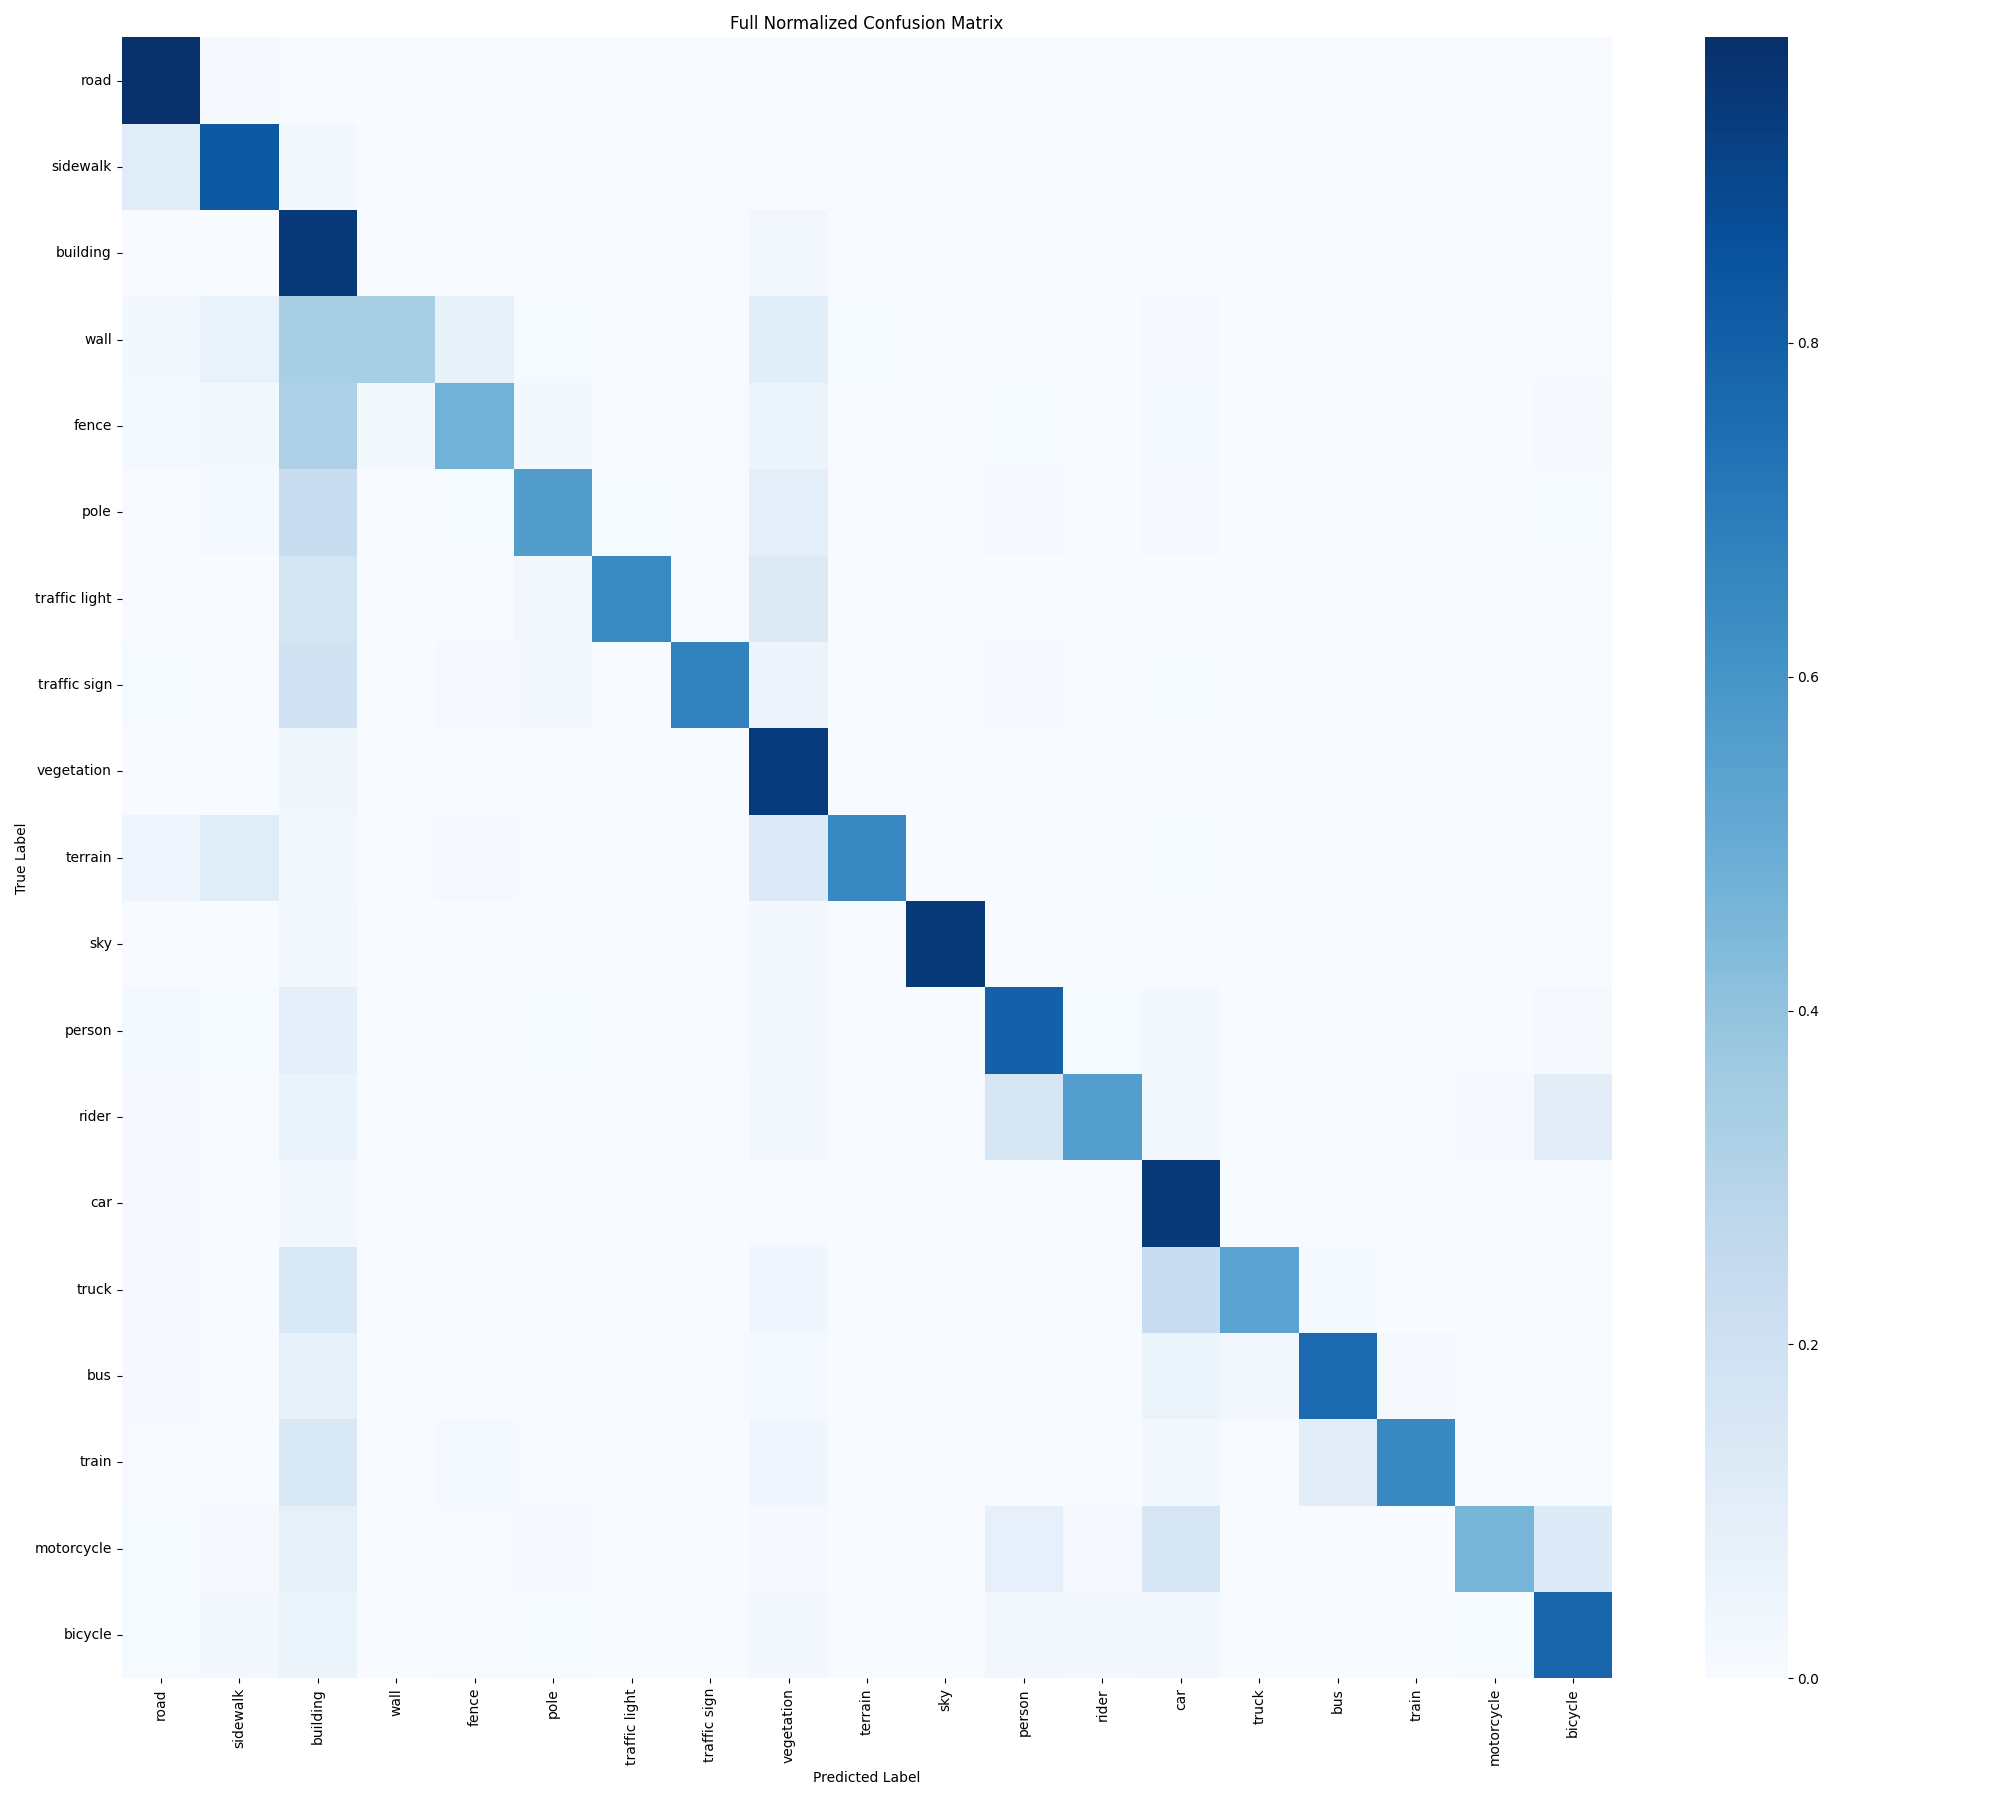
\includegraphics[width=0.8\textwidth]{outputs/deeplabv3plus_test_results/full_confusion_matrix.png}
    \caption{Confusion matrix for the segmentation results, illustrating the distribution of predicted classes versus ground truth}
    \label{fig:confusion_matrix}
\end{figure}

\begin{figure}[htbp]
    \centering
    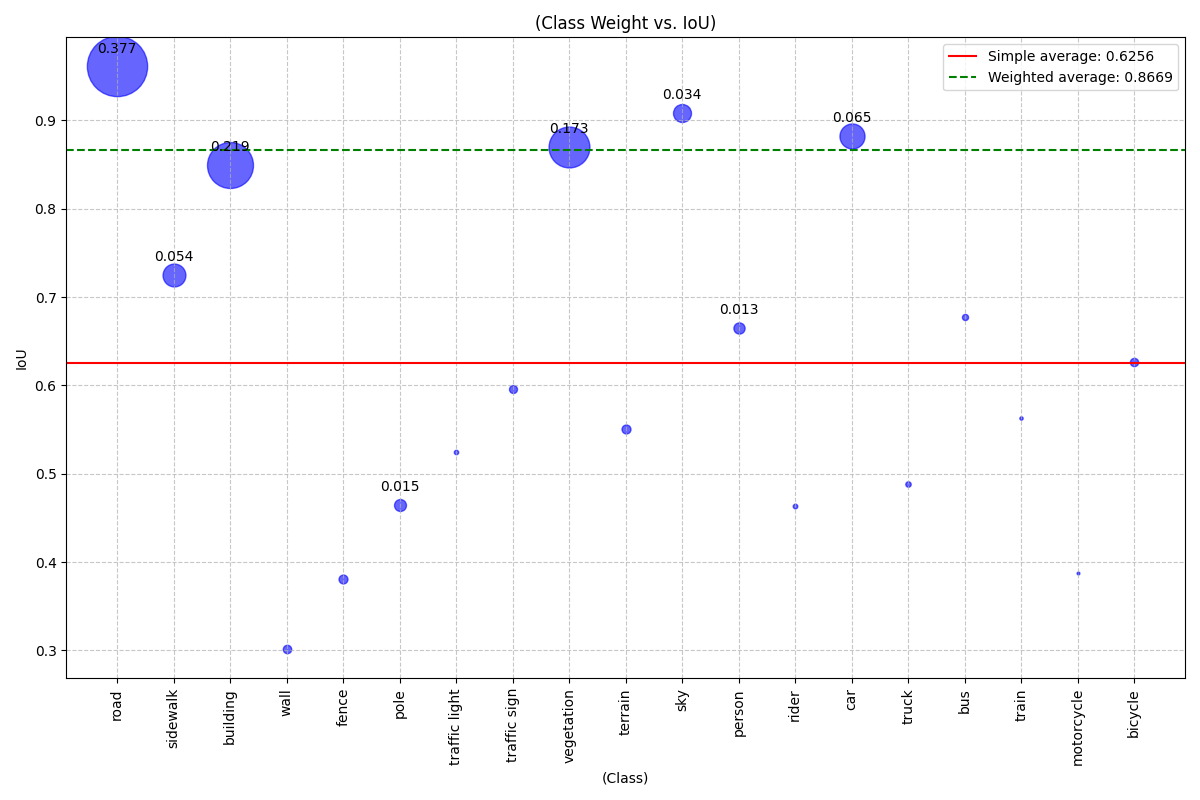
\includegraphics[width=0.8\textwidth]{outputs/deeplabv3plus_test_results/class_weight_vs_iou.png}
    \caption{Correlation between class weights and IoU scores, showing the relationship between class frequency and segmentation performance}
    \label{fig:class_weight_vs_iou}
\end{figure}

\section{Acknowledgements}
I would like to acknowledge the authors of the DeepLabV3+ architecture, whose work provided the foundation for this implementation. I also utilized GitHub Copilot as a programming assistant to help streamline code development and debugging. 

\end{document}